\documentclass[Main]{subfiles}
\begin{document}

\chapter{Conclusion}

\section{Conclusion}
Java RMI (Remote Method Invocation) can be used to invoke methods of
objects in another Java Virtual Machine (JVM). The JVM can be on the
local host or another host. RMI allows the client to invoke remote methods in the server as if the remote object were contained on the client host, from the programmer's perspective.\\When a client calls a method in a remote object, instead of letting the Java runtime take care of the call as it would for regular Java objects, the RMI runtime system takes over and routes the call over the network to the remote object. None of the underlying communication is visible to the programmer.

Java RMI are used in distributed systems. Distributed systems have multiple PC's running multiple processes and theses processes have to cooperate in solving a given task. Handling all these processes in cooperating, its important that there is a leader, which all process can interact with. To find a leader between all the processes, there are different leader election algoritms which could be used, e.g. Bully algoritm or The Chang and Roberts algorithm. The leader election algoritms are used when the systems starts and when a leader process have failed or retires on purpose. This mean that the system can go on, even if a given leader process is failing.

\section{Discussion}

Maybe we can use some of this to argue why to use Java RMI:
\begin{figure}[H]
\centering
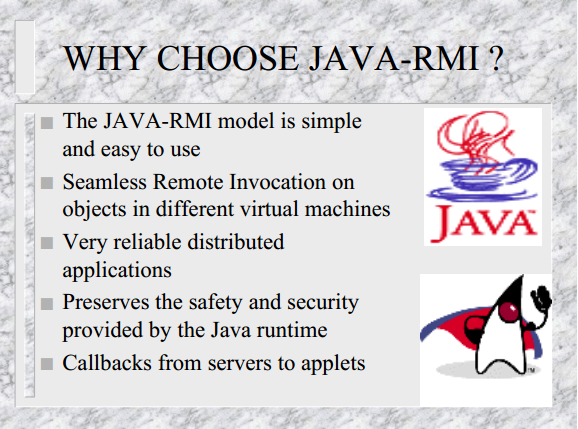
\includegraphics[scale=1]{Figurer/discussion.png}
\caption{From: http://www.uniforum.chi.il.us/slides/javarmi/javarmi.pdf}
\end{figure}


\section{Perspectives}
What are the perspectives on the technology and your prototype? 


\end{document} 